% vim: set spelllang=fr foldmethod=marker:
\section{Comparaison numérique des méthodes de sélection\index{selection@sélection}}

    \subsection{Mise en place des simulations}

        %\subsubsection{Modèle utilisé}

Le modèle utilisé dans cette section est similaire à celui employé au \chapref{sa} (défini en \ssref{sa:ssec:modelsim}).
Tout comme alors, le logiciel \nsii a été mis en œuvre.
Le cluster est composé d'une grille carrée de cent capteurs, avec le \ch en son centre (soit cent-un capteurs au total; voir \figref{sa:fig:grille}).

La \tabref{sd:table:param} récapitule les principaux paramètres impliqués dans l'exécution des instances.
\begin{table}[ht]
    \centering
    \caption{Paramètres de simulation}\label{sd:table:param}
    \medskip
    \begin{tabu}to \textwidth {l@{\hspace{.5em}}X[c]}
        \toprule
        \textsc{Paramètre}                                          & \textsc{Valeur}        \\
        \midrule
        Durée de la simulation                                      & 3\,600~secondes        \\
        Nombre de capteurs                                          & 100 (+~\ch)            \\
        Nombre de \cns                                              & 7--10 (selon scénario) \\
        Nombre de nœuds compromis                                   & 1                      \\
        Fréquence de renouvellement des \cns                        & toutes les 10~secondes \\
        Durée de la période initiale pour la sélection démocratique & 60~secondes            \\
        Mobilité des nœuds                                          & nulle                  \\
    \end{tabu}\index{renouvellement}\index{selection@sélection!election democratique@élection démocratique}
    \begin{tabu}to \textwidth {l X[c] X[c]}
        \midrule
        \multirow{2}{*}{\textsc{Paramètre}} & \textsc{Valeur}                    & \textsc{Valeur}           \\
                                            & \textsc{(nœuds normaux)}           & \textsc{(nœud compromis)} \\
        \midrule
        Taux d'émission                     & 1~ko/s                             & 35~ko/s                   \\
        Taille des paquets                  & 500~octets                         & 100~octets                \\
        Intervalle                          & aléatoire (\textsc{Poisson})       & constant                  \\
        Cons. énergétique en émission       & 0,660~W                            & 0,660~W                   \\
        Cons. énergétique en réception      & 0,395~W                            & non prise en compte       \\
        Quantité initiale d'énergie         & 10~\joule\ --- $\infty$ (sel. sc.) & $\infty$                  \\
        \bottomrule
    \end{tabu}\index{renouvellement}
\end{table}

\newcommand\idstat{\textsf{\#Stat10}\xspace}
\newcommand\idrand{\textsf{\#Aléa10}\xspace}
\newcommand\ideres{\textsf{\#ÉRes10}\xspace}
\newcommand\iddemx{\textsf{\#Démc10}\xspace}
\newcommand\iddems{\textsf{\#Démc07}\xspace}
Dans les chapitres précédents, le but des simulations était de souligner les apports des nouvelles solutions proposées par rapport aux éléments antérieurs.
Ici, l'objectif consiste plutôt à comparer tous les scénarios que nous avons définis au cours des trois chapitres sur les processus de sélection\index{selection@sélection}.
Un «scénario» se caractérise donc avant tout par le choix d'un processus de \idx{renouvellement} des \cns, mais aussi par le nombre de \cns sélectionnés à chaque tour, et par le montant d'énergie initialement attribué aux capteurs.
Chaque graphe présente, pour un montant d'énergie initiale donné, les valeurs obtenues pour cinq scénarios distincts, auxquels nous attribuons des identifiants pour pouvoir nous y référer plus facilement par la suite:
\begin{itemize}
    \item l'un ne comporte aucun \idx{renouvellement} des dix~\cns (il s'agit de la méthode dite «\underline{stat}ique», que nous nommons dans cette section \idstat);
    \item l'un se base sur un processus de \idx{renouvellement} \underline{aléa}toire tel que présenté au \chapref{sa} (\idrand);
    \item l'un se base sur un \idx{renouvellement} selon l'\underline{é}nergie \underline{rés}iduelle (avec usage de \vns) tel que présenté au \chapref{se} (\ideres);
    \item les deux derniers se basent sur le mécanisme d'élection \underline{dém}o\underline{c}ratique\index{selection@sélection!election democratique@élection démocratique} abordé dans ce chapitre:
        \begin{itemize}
            \item l'un avec dix~\cns (\iddemx),
            \item l'autre avec sept~\cns seulement, afin d'observer l'effet de la diminution du nombre de nœuds sélectionnés (\iddems).
        \end{itemize}
\end{itemize}
Sauf indication contraire, tous les résultats numériques présentés dans cette section sont des moyennes calculées à partir des valeurs de dix instances distinctes (pour chaque scénario).
Ces instances sont différenciées par les valeurs utilisées pour initialiser le générateur de nombres pseudo-aléatoires de \nsii, et (le cas échéant) celui utilisé par les nœuds pour la sélection\index{selection@sélection} des \cns.

Les moyennes sur les capteurs sont calculées à partir des valeurs des quatre-vingt-dix-neuf nœuds «sains».
Le \ch ainsi que le nœud compromis sont dotés d'une réserve d'énergie illimitée pour les simulations:
\begin{itemize}
    \item le \ch parce qu'il est indispensable au fonctionnement du cluster, et que sur une instance réelle, l'épuisement de sa batterie se traduirait par la désignation immédiate d'un remplaçant; de plus, il reçoit les paquets «utiles» de tous les nœuds, et sa consommation en énergie, très importante, viendrait «fausser» les moyennes que nous cherchons à étudier ici;
    \item le nœud compromis parce que nous ne souhaitons pas qu'il arrête d'émettre au cours du déroulement de notre scénario; et parce que les nombreux paquets qu'il émet lui font là aussi dépenser une énergie qui viendrait fausser les moyennes observées. Outre le contexte des simulations, il est à noter qu'un tel cas est plausible, par exemple, si l'attaquant substitue au nœud ciblé un appareil plus puissant (un ordinateur portable par exemple) sur une longue durée: le nœud compromis peut alors se retrouver affranchi des contraintes en énergie auxquelles sont soumis les autres capteurs.
\end{itemize}

        %\subsubsection{Choix du simulateur}

%Le simulateur utilisé au \chapref{sa} est \nsii~\cite{ns2}; celui employé au \chapref{se} est \nsiii~\cite{ns3}.
%\nsiii est une version plus récente de \nsii.
%Basé sur les mêmes mécanismes, le logiciel a été complètement réécrit, et les langages utilisés pour définir les scénarios de simulation ne sont plus les mêmes (Tcl pour \nsii, \cpp (éventuellement Python) pour \nsiii).
%Ce changement radical a pour conséquence l'absence de compatibilité descendante avec \nsii.

%Il semble nécessaire d'expliquer ici en quelques mots le choix des logiciels utilisés.
%Nous avons commencé à travailler sur \nsii, sans vraiment étudier d'alternative dans un premier temps.
%Cependant les travaux de simulation présentés aux chapitres~\ref{chap:sa} et~\ref{chap:se} n'ont pas été réalisé d'une seule traite, mais avec plusieurs mois d'écart.
%Durant cette période, nous avons pensé abandonner \nsii pour nous tourner vers \nsiii, plus récent, mieux conçu, mieux documenté (bien que moins complet à ce jour, mais cela ne nous a pas porté préjudice pour les simulations réalisées).

%Malheureusement, nous nous sommes heurtés à des problèmes de performances: une instance d'une durée (virtuelle) d'une demi-heure, sous \nsiii, nous a pris une semaine entière à exécuter, sur un ordinateur récent.
%Malgré nos requêtes sur la liste ainsi que sur le canal de discussion associés au simulateur, nous n'avons pas réussi à contourner cet écueil.
%Nous ne savons toujours pas, à la publication de cet ouvrage, si le problème vient d'une erreur introduite avec notre code, ou bien s'il s'avère simplement que \nsiii se prête mal à ce type de scénarios.
%Certaines sources semblent affirmer qu'avec \nsiii, «le passage à l'échelle n'est pas efficace pour les WSN»\,\footnote{«\textit{[\nsiiinxs] does not scale well for WSNs}»~\cite{AAAHN12}}, ce qui tendrait à conforter la seconde hypothèse.

%Devant la durée très (trop) importante de l'exécution des simulations désirées, nous sommes revenus vers \nsii pour comparer dans ce chapitre l'ensemble des processus de sélection proposés.

\pagebreak %%%%%%%%%%%%%%%%%%%%%%%%%%%%%%%%%%%%%%%%%%%%%%%%%%%%%%%%%%%%%%%%%%%%

    \subsection{Résultats numériques}

        \subsubsection{Consommation énergétique}

Une première série d'instances a été exécutée en attribuant une quantité d'énergie «illimitée» aux capteurs au regard de la durée virtuelle de la simulation.
Ceci permet d'observer la quantité d'énergie moyenne consommée par les nœuds lorsque chaque méthode de sélection\index{selection@sélection} des \cns est déployée dans le cluster.
La \figref{sd:fig:cons-inf} présente les valeurs obtenues.
On peut y observer une consommation quasiment identique entre les méthodes \idstat et \idrand, puisque le \idx{renouvellement} en soi, à l'aide de la sélection pseudo-aléatoire\index{selection@sélection!sélection aléatoire} des \cns, ne représente pratiquement aucun cout additionnel.
Les méthodes \ideres et \iddemx consomment toutes deux davantage, à cause des mécanismes mis en place pour récolter les valeurs de l'énergie résiduels des nœuds, et pour assurer la \secu du processus.
\begin{figure}[!hb]
    \centering
    \includegraphics{\chapterfig/plot_sd_consumptionXtime.pdf}
    \caption[Moyenne de l'énergie consommée par les capteurs au cours du temps]{Moyenne de l'énergie consommée par les capteurs au cours du temps (énergie initiale: $\infty$)}\label{sd:fig:cons-inf}
\end{figure}

La méthode \iddemx est plus couteuse au départ, ce qui est parfaitement visible en agrandissant la vue sur l'origine du repère comme le fait la \figref{sd:fig:cons-inf-zoom}.
\begin{figure}[p]
    \centering
    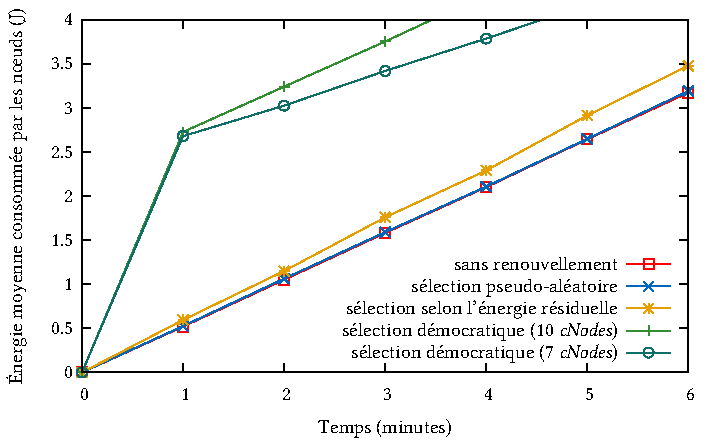
\includegraphics{\chapterfig/plot_sd_consumptionXtime_zoom10.pdf}
    \caption[Moyenne de l'énergie consommée par les capteurs au cours du temps: agrandissement de la vue près de l'origine du repère]{Moyenne de l'énergie consommée par les capteurs au cours du temps: agrandissement de la vue près de l'origine du repère (énergie initiale: $\infty$)}\label{sd:fig:cons-inf-zoom}
\end{figure}
Les deux scénarios basés sur la sélection démocratique\index{selection@sélection!election democratique@élection démocratique} voient leur quantité d'énergie consommée augmenter très rapidement pendant la première minute de la simulation, qui correspond à la période initiale (où tous les nœuds agissent comme des \cns en plus de prendre des mesures, d'où la consommation accrue).
En revanche, on observe une inversion entre \ideres et \iddemx peu avant 40~minutes, signe que sur le long terme, \iddemx consomme moins d'énergie que l'usage des \vns.
\iddems, quant à elle, est à terme la méthode la plus économe en énergie: ceci met en avant le poids des \cns dans la consommation totale en énergie du cluster.
Moins on utilise de \cns, moins l'énergie consommée est importante (comme indiqué déjà par les résultats du \chapref{sa}, en \sref{sa:sec:resultats}).

\begin{figure}[p]
    \centering
    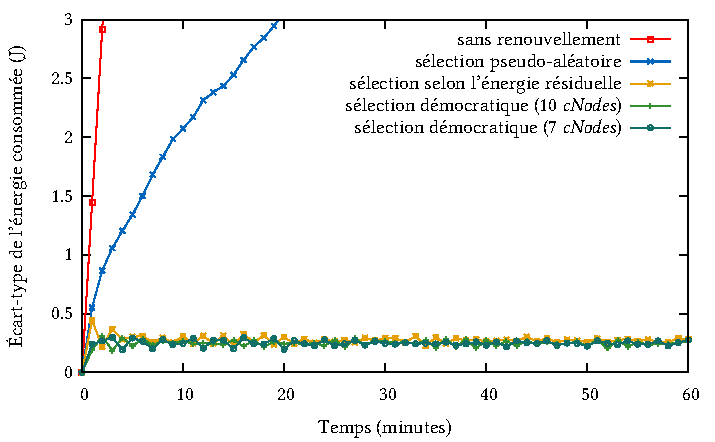
\includegraphics{\chapterfig/plot_sd_stddevXtime.pdf}
    \caption[Écart-type moyen pour l'énergie consommée par les capteurs au cours du temps]{Écart-type moyen pour l'énergie consommée par les capteurs au cours du temps (énergie initiale: $\infty$)}\label{sd:fig:stddev-inf}
\end{figure}
\pagebreak %%%%%%%%%%%%%%%%%%%%%%%%%%%%%%%%%%%%%%%%%%%%%%%%%%%%%%%%%%%%%%%%%%%%
Les méthodes qui prennent en compte l'énergie résiduelle (\ideres, \iddemx) sont donc, pour un nombre de \cns équivalent, plus gourmandes en énergie; mais il est aussi intéressant d'étudier la répartition de la charge qu'elles apportent au cluster.
La \figref{sd:fig:stddev-inf} présente les écarts-types obtenus, au court des mêmes simulations, pour les cinq~scénarios.
On peut y observer que pour \idstat se crée un déséquilibre croissant (de façon linéaire): puisque les \cns sont toujours les mêmes, ce sont toujours les mêmes capteurs qui consomment l'énergie, creusent l'écart, et diminuent l'équilibre du réseau.
Pour la méthode \idrand, l'écart monte rapidement, mais ralentit et se stabilise peu à peu (la valeur (toujours croissante) en fin de simulation, non apparente sur la figure, est à un peu plus de 6~\joule): la loi des grands nombres fait que (sous réserve de l'utilisation d'un générateur de nombres pseudo-aléatoires bien conçu), lorsque la durée de simulation s'allonge, tous les nœuds sont sélectionnés un nombre de fois approximativement identique.
Mais cet écart demeure très important à côté de celui de \ideres, \iddemx et \iddems, très proche de zéro: ces méthodes assurent une très bonne répartition de la consommation en énergie dans le cluster, ce qui, pour rappel, constituait leur objectif initial.

        \subsubsection{Durée de vie du réseau}
Une deuxième et une troisième série d'instances ont été réalisées pour analyser la durée de vie du réseau ainsi que le taux de détection de l'attaque.
C'est d'abord la durée de vie des capteurs qui est étudiée ici.
Son évolution a été observée au cours du temps, dans un cluster doté d'une énergie initiale de 10~\joule (deuxième série) puis de 20~\joule (troisième série) par nœuds.
Ce montant d'énergie est suffisamment bas pour observer l'arrêt de la plupart des nœuds au cours de l'heure virtuelle simulée.

La \figref{sd:fig:nbnodes-10J} présente ainsi le nombre de nœuds encore en activité en fonction du temps, lorsqu'une énergie de 10~\joule a initialement été affectée aux capteurs.
\begin{figure}[!b]
    \centering
    \includegraphics{\chapterfig/plot_sd_nbnodesXtime_10J.pdf}
    \caption{Nombre de nœuds en activité au cours du temps pour un montant d'énergie initiale de 10~\joule}\label{sd:fig:nbnodes-10J}
\end{figure}
La méthode \idstat est de loin celle qui conserve ses nœuds le plus longtemps.
Et pour cause: comme les \cns ne sont pas renouvelés, les 10~capteurs initialement sélectionnés sont les seuls à consommer de manière accrue, et à vider (très rapidement, d'ailleurs) leur batterie.
Le dixième nœud à épuiser sa batterie s'arrête longtemps après le neuvième: cela est dû au calcul des moyennes sur plusieurs instances.
Il arrive en effet que le nœud compromis soit sélectionné parmi les \cns; mais comme sont énergie n'apparait pas sur la courbe, les résultats sont ceux obtenus pour seulement 9~\cns sélectionnés dans ce cas, et le dixième nœud à tomber hors service est un nœud normal qui survit largement à l'heure que dure la simulation.

La méthode de \idx{renouvellement} aléatoire \idrand est efficace pour préserver l'énergie dans le cluster.
Comme le nombre de \cns sélectionnés est statistiquement un pourcentage du nombre de nœuds dans le cluster (on sélectionne $k$ nœuds de façon aléatoire, sans regarder s'ils sont encore en vie), la réduction du nombre de nœuds n'entraine pas l'accélération de la consommation.
De plus, la méthode est simple à mettre en œuvre, et ne nécessite que peu d'échanges de données de contrôle.

Les méthodes \ideres, \iddemx et \iddems en revanche ne sont pas aussi efficaces dans ce contexte.
L'énergie est consommée plus rapidement que ce soit à cause de la période initiale (\iddemx et \iddems) ou bien par le recours aux \vns.
Il en résulte un arrêt plus rapide qu'avec \idrand.
Et surtout, ce premier arrêt est très rapidement suivi par celui des autres capteurs, ceci pour les deux raisons suivantes:
\begin{itemize}
    \item l'écart-type de l'énergie consommée étant très faible dans le cluster, tous les capteurs ont à peu près la même consommation, et leur énergie résiduelle atteint un niveau nul au même moment;
    \item le fait de sélectionner les 10~\cns parmi les nœuds ayant le plus d'énergie résiduelle provoque la désignation systématique de 10~\cns, puisque l'on ne risque pas de désigner «par erreur» des nœuds dont la batterie seraient épuisée. Lorsque les premiers nœuds s'arrêtent, le pourcentage de \cns par rapport aux capteurs non sélectionnés augmente donc mécaniquement, contrairement à la méthode \idrand, et pousse les nœuds restant à vider rapidement leur batterie.
\end{itemize}

On peut observer que de ces méthodes basées sur l'énergie résiduelle, \iddems est la plus efficace ici (puisqu'elle met en jeu moins de \cns), tandis que \ideres se classe deuxième et \iddemx dernière, pénalisée par l'énergie consommée au cours de sa période initiale.
Pourtant l'écart creusé par cette période initiale peut être rattrapé.
C'est ce que montre la \figref{sd:fig:nbnodes-20J},
\begin{figure}[!t]
    \centering
    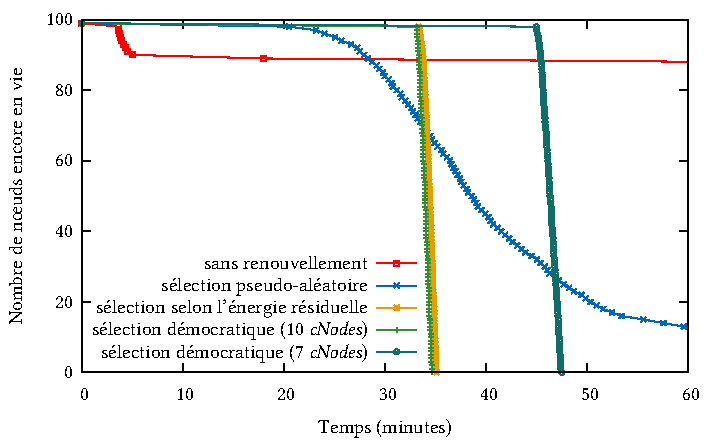
\includegraphics{\chapterfig/plot_sd_nbnodesXtime_20J.pdf}
    \caption{Nombre de nœuds en activité au cours du temps pour un montant d'énergie initiale de 20~\joule}\label{sd:fig:nbnodes-20J}
\end{figure}
qui reprend les mêmes scénarios, mais développés sur la consommation des 20~\joule (au lieu de 10~\joule) initialement attribués au capteurs: \iddemx et \ideres sont quasiment à égalité dans ce cas.
On retrouve un comportement à peu près identique pour \idstat et \idrand par rapport à la \figref{sd:fig:nbnodes-10J}, mais bien évidemment avec une durée d'épuisement des nœuds doublée.
Tout comme \iddemx grignote du terrain sur \ideres, on observe que \iddems gagne en efficacité en comparaison de \idrand: avec 10~\joule d'énergie initiale, les nœuds s'épuisent d'un coup pour \iddems peu après 20~minutes, alors qu'il reste près de la moitié des nœuds pour la méthode \idrand au même instant.
Tandis qu'avec 20~\joule d'énergie initiale, l'écart créé par la période initiale de \iddems a été en partie rattrapé, et lorsque le nombre de nœuds chute peu avant les 50~minutes de simulation, près de trois quarts des capteurs sont épuisés avec \idrand.
Avec une quantité plus élevée d'énergie initiale, le nombre inférieur de \cns ferait rapidement la différence en faveur de la méthode \iddems.

        \subsubsection{Taux de détection}
Le nombre de nœuds en mesure de détecter l'attaque du nœud compromis est directement lié au nombre de nœuds encore en activité dans le réseau, puisque les capteurs ayant épuisé leur batterie n'ont plus aucune chance de mener à bien l'opération de surveillance.
À titre indicatif, la \figref{sd:fig:detec-one-10J} représente le taux de détection à chaque phase (de 10~secondes), sur une seule instance (pas de moyenne, donc), pour chaque méthode de sélection\index{selection@sélection}, l'énergie initiale assignée aux capteurs étant de 10~\joule.
\begin{figure}[p]
    \centering
    \includegraphics{\chapterfig/plot_sd_detectionXtime-single_10J.pdf}
    \caption[Taux de détection au cours du temps (énergie initiale: 10~\joule; valeurs sur une seule instance)]{Taux de détection, pour chaque processus de sélection\index{selection@sélection}, au cours du temps (énergie initiale: 10~\joule; valeurs sur une seule instance)}\label{sd:fig:detec-one-10J}
\end{figure}
En dehors d'un intérêt artistique certain, ces courbes permettent d'observer les extremums atteints, mais sont très peu lisibles.
La \figref{sd:fig:detec-min-10J} reprend donc ces valeurs, lissées une première fois en calculant la moyenne du nombre d'attaques détectées par les différentes instances (10~par scénario), puis une seconde fois sur une séquence d'une minute (donc 6~phases de 10~secondes).
\begin{figure}[p]
    \centering
    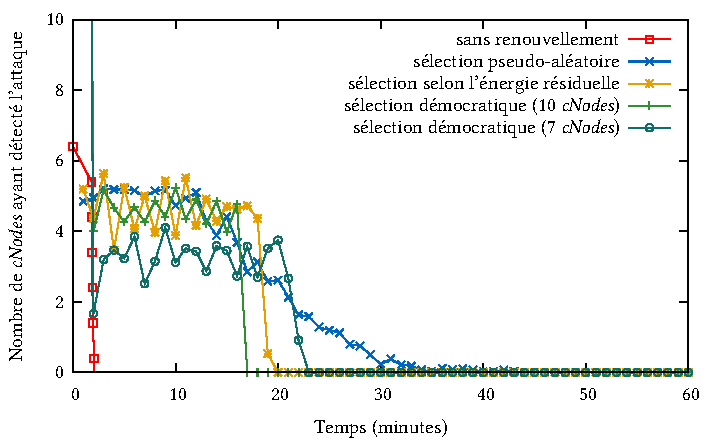
\includegraphics{\chapterfig/plot_sd_detectionXtime-minute_10J.pdf}
    \caption[Taux de détection au cours du temps (énergie initiale: 10~\joule)]{Taux de détection, pour chaque processus de sélection\index{selection@sélection}, au cours du temps (énergie initiale: 10~\joule; valeurs lissées sur une durée d'une minute)}\label{sd:fig:detec-min-10J}
\end{figure}
On observe que pour la méthode \idstat, la détection chute très rapidement à zéro; en fait dès que les \cns d'origine, non renouvelés, ont consommé leurs réserves.
Les méthodes \idrand, \ideres et \iddemx ont toutes les trois un bon niveau de détection, avec en moyenne 5~\cns parmi les 10~sélectionnés qui repèrent l'attaque tant que la plupart des nœuds sont en activité.
La méthode \iddems tourne plutôt sur une moyenne de 3~à 4~\cns détectant l'attaque, mais sur un total de~7.
La détection se poursuit en revanche un peu plus longtemps que sur \ideres et \iddemx, puisque les nœuds consomment au total moins d'énergie.
Les maigres réservent accordées ne lui permettent pas d'avoir le temps, en revanche, de passer devant la sélection aléatoire\index{selection@sélection!sélection aléatoire} \idrand, qui détecte encore parfois l'attaque au-delà de 30~minutes de simulation.

Il est à noter que la position du nœud compromis a une influence directe sur le nombre de nœuds détectant l'attaque.
Suivant le nombre de voisins directs qu'il possède, ce nœud a plus ou moins de chances d'être détecté.
Pour toutes les simulations réalisées dans cette partie, le nœud compromis occupe la position indiquée sur la \figref{sd:fig:neighbors}, et possède (en dehors du \ch) un total de 61~voisins directs, qui sont autant de \cns en puissance capables de détecter l'attaque\,\footnote{Le modèle de couche physique utilisé pour les simulations ne comporte pas de composante aléatoire: hors collisions\index{collision}, soit deux nœuds sont à portée et reçoivent tous leurs messages sans pertes dues à l'affaiblissement, soit l'échange est systématiquement impossible.}.
Toutefois, «surveillance» n'est pas systématiquement égale à «détection», et un \cn à portée peut échouer à détecter l'attaque (s'il manque trop de paquets à cause des collisions\index{collision}, par exemple).
\begin{figure}[p]
    \centering
    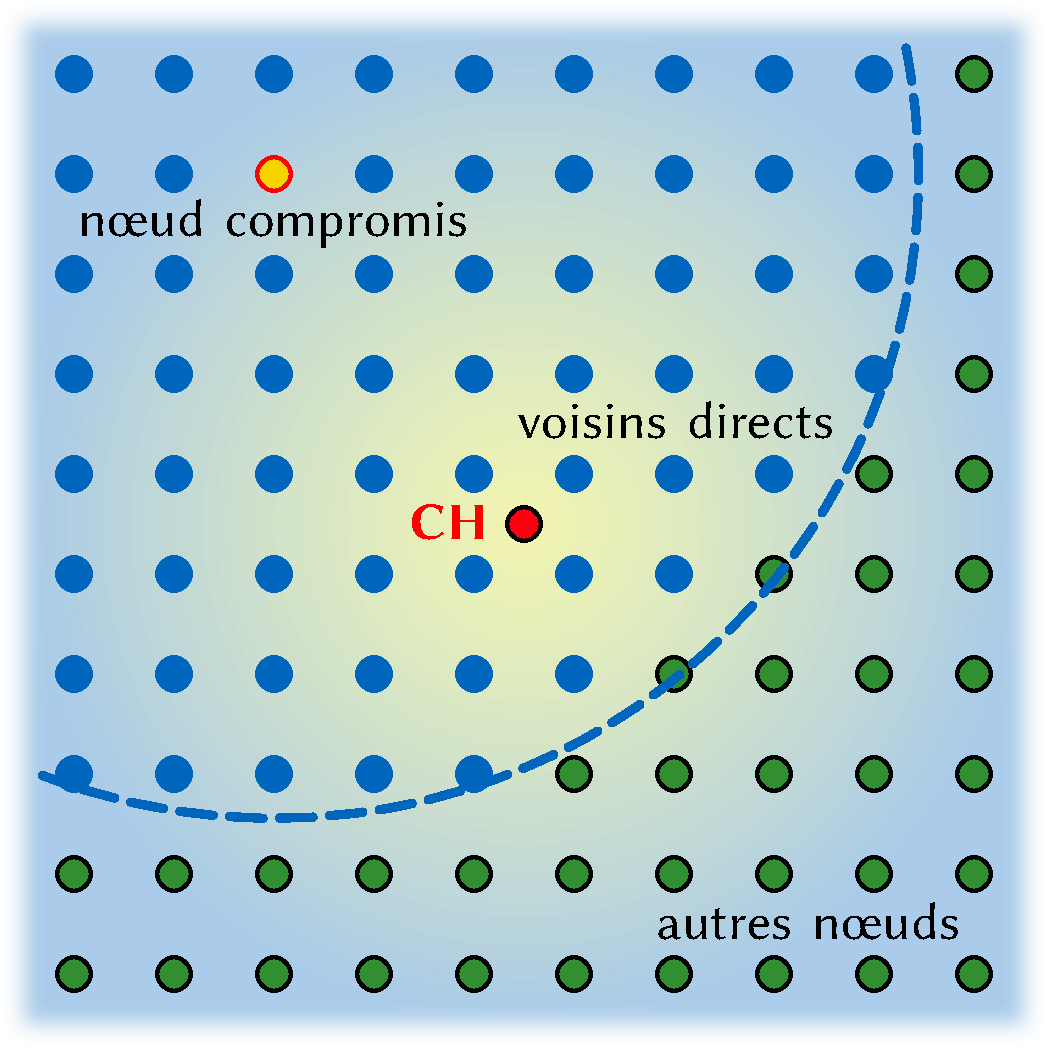
\includegraphics[width=6.5cm]{\chapterfig/WSN_neighbors.pdf}
    \caption[Schéma du cluster représentant la position des 61~voisins directs du nœud compromis]{Schéma du cluster représentant la position des soixante-et-un voisins directs (en bleu) du nœud compromis (en jaune) tels que définis dans les simulations réalisées}\label{sd:fig:neighbors}
\end{figure}

%CALCUL : probabilité que n cNodes parmi les 10 soient piochés parmi les NON voisins du nœud 12 compromis (code JavaScript)
%function f(n) {
  %if (n<=1)
    %return 1;
  %else
    %return f(n-1)*n;
%}
%function p(k) {
  %m=61;
  %N=100;
  %n=10;
  %Nm=N-m;
  %nk=n-k;
  %ckm = f(m)/(f(k)*f(m-k));
  %cnkNm = f(Nm)/(f(nk)*f(Nm-nk));
  %cnN = f(N)/(f(n)*f(N-n));
  %return ckm*cnkNm/cnN;
%}
%var sum=0;
%for (var i=0;i<=10;i++) {
  %sum+=p(i);
  %console.log(i, p(i)*100);
%}

%Résultats (%) :
%0 0.0036726402702378143 ~ 1/27228
%1 0.07467701882816889
%2 0.6504127446324387
%3 3.19786266110949
%4 9.835850306139795
%5 19.78741649823418
%6 26.383221997645574
%7 23.032971585246138
%8 12.605883097330656
%9 3.907086574026461
%10 0.5209448765368615
Cette remarque sur la disposition permet de réaliser une seconde observation sur le nombre de chances que possède le nœud compromis d'échapper, à propos de la couverture géographique, à la surveillance des \cns.
Avec les méthodes \ideres, \iddemx et \iddems, cette chance est nulle (tant qu'il reste suffisamment de nœuds actifs), puisque les méthodes employées spécifient que chaque nœud du cluster doit être couvert par au moins deux \cns.
Mais le processus \idrand, en revanche, est tel que pour certaines phases, tous les \cns peuvent être sélectionnés parmi l'ensemble des nœuds non~voisins du nœud compromis.
Cette probabilité se calcule.
La répartition des \cns, lors du processus de sélection aléatoire\index{selection@sélection!sélection aléatoire}, suit une loi de probabilité hypergéométrique.
Il est possible de calculer la probabilité pour que $k$ \cns sur les $n=10$ soient choisis parmi les $m=61$ voisins directs du nœud compromis, sur un total de $N=100$ candidats, à l'aide de la formule suivante:
$$P(k) = \frac{{m\choose k}{N-m\choose n-k}}{{N\choose n}}=
\frac{m!}{k!\,(m-k)!}\times\frac{(N-m)!}{(n-k)!\,((N-m)-(n-k))!}\times\frac{n!\,(N-n)!}{N!}$$
La probabilité que le nœud compromis ne soit surveillé par aucun \cn est donc de:
%\begin{align*}
    %P(0)&=\frac{61!}{0!\,(61-0)!}\times\frac{(100-61)!}{(10-0)!\,((100-61)-(10-0))!}\times\frac{10!\,(100-10)!}{100!}\\
        %&\approx3,6\times10^{-5}\approx1/27228
%\end{align*}
$$P(k=0)\approx3,6\times10^{-5}\approx1/27228$$
Elle est très faible; mais il faut tenir compte encore une fois du fait que la surveillance peut échouer et ne pas mener à la détection de l'attaque, que ce soit en raison d'un nombre important de collisions\index{collision} dans le cluster qui viendrait perturber l'écoute du trafic, ou parce que sur une période donnée le capteur compromis a émis légèrement moins de paquets que d'habitude et que le seuil n'est pas atteint pour toutes les sentinelles.

La \figref{sd:fig:detec-min-20J} présente les mêmes résultats, pour une énergie initiale de 20~\joule assignée aux capteurs.
Les résultats, de manière prévisible, montrent que la durée de surveillance a à peu près doublé pour chaque méthode, avec une augmentation des performances pour \iddemx et \iddems (par rapport à la figure précédente), qui ont eu l'occasion de «rattraper» davantage l'écart creusé sur la consommation en énergie lors de leur période initiale.
Avec encore un peu plus d'énergie allouée au début de la simulation, \iddemx permettrait au capteurs de maintenir la détection plus longtemps que \ideres, et à terme tendrait vers une efficacité presque équivalente à \idrand, sans la rattraper toutefois en raison d'un volume de données de contrôle légèrement supérieur.
\begin{figure}[p]
    \centering
    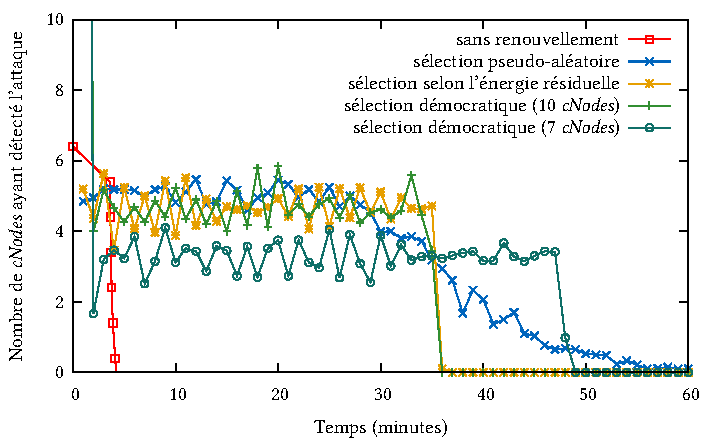
\includegraphics{\chapterfig/plot_sd_detectionXtime-minute_20J.pdf}
    \caption[Taux de détection au cours du temps (énergie initiale: 20~\joule)]{Taux de détection, pour chaque processus de sélection\index{selection@sélection}, au cours du temps (énergie initiale: 20~\joule; valeurs lissées sur une durée d'une minute)}\label{sd:fig:detec-min-20J}
\end{figure}

Au vu des caractéristiques obtenues pour chaque méthode, nous pouvons à présent résumer leurs avantages et leurs inconvénients, et en déduire des recommandations d'usage selon la configuration du réseau déployé.
\pagebreak %%%%%%%%%%%%%%%%%%%%%%%%%%%%%%%%%%%%%%%%%%%%%%%%%%%%%%%%%%%%%%%%%%%%
